%\documentclass[a4paper]{article}
\usepackage[utf8]{inputenc}
\usepackage[spanish, es-tabla, es-noshorthands]{babel}
\usepackage[table,xcdraw]{xcolor}
\usepackage[a4paper, footnotesep = 1cm, width=22cm, top=2.5cm, height=25cm, textwidth=20cm, textheight=25cm]{geometry}
%\geometry{showframe}

\usepackage{tikz}
\usepackage{amsmath}
\usepackage{amsfonts}
\usepackage{amssymb}
\usepackage{float}
\usepackage{graphicx}
\usepackage{caption}
\usepackage{subcaption}
\usepackage{multicol}
\usepackage{multirow}
\usepackage{wrapfig}
\setlength{\doublerulesep}{\arrayrulewidth}
\usepackage{booktabs}

\usepackage{hyperref}
\hypersetup{
    colorlinks=true,
    linkcolor=blue,
    filecolor=magenta,      
    urlcolor=blue,
    citecolor=blue,    
}

\newcommand{\note}[1]{
	\begin{center}
		\huge{ \textcolor{red}{#1} }
	\end{center}
}

\setcounter{topnumber}{2}
\setcounter{bottomnumber}{2}
\setcounter{totalnumber}{4}
\renewcommand{\topfraction}{0.85}
\renewcommand{\bottomfraction}{0.85}
\renewcommand{\textfraction}{0.15}
\renewcommand{\floatpagefraction}{0.8}
\renewcommand{\textfraction}{0.1}
\setlength{\floatsep}{5pt plus 2pt minus 2pt}
\setlength{\textfloatsep}{5pt plus 2pt minus 2pt}
\setlength{\intextsep}{5pt plus 2pt minus 2pt}

\newcommand{\quotes}[1]{``#1''}
\usepackage{array}
\newcolumntype{C}[1]{>{\centering\let\newline\\\arraybackslash\hspace{0pt}}m{#1}}
\usepackage[american]{circuitikz}
\usetikzlibrary{calc}
\usepackage{fancyhdr}
\usepackage{units} 

\graphicspath{{../Ejercicio-1/}{../Ejercicio-2/}{../Ejercicio-3/}{../Ejercicio-4/}{../ParteI/}{../ParteII/}{../ParteIII/}{../ParteIV/}}

\pagestyle{fancy}
\fancyhf{}
\lhead{22.14 - Electrónica IV}
\rhead{Mechoulam, Lambertucci, Londero}
\rfoot{Página \thepage}

%
%\begin{document}

\subsection{Diseño de placa}
Se diseño la placa en multiperforada, teniendo la posibilidad de medir la tensión en los pines de compensación, drain, gate, primario, secundario y en el pin no inversor. Tambíen es posible cambiar la carga del circuito, y la tensión de salida.

Se colocaron a la salida varios capacitores en paralelo, teniendo distintas tecnologías (electrolíticos, cerámicos) para bajar la ESR, al igual que para subir la capacidad de salida. 

%Se tuvo en cuenta no unir islas con estaño sino siempre con cables. 
El sistema, si bien fue diseñado en modo continuo, trabaja en modo discontinuo debido a la baja corriente de salida que es pedida por la carga. Aún si se quisiese, no podría trabajar en modo continuo debido a que la corriente necesaria para que este trabaje en modo continua resultaría en la saturación del transformador lo cual no es deseable.

\begin{figure}[H]
	\centering
	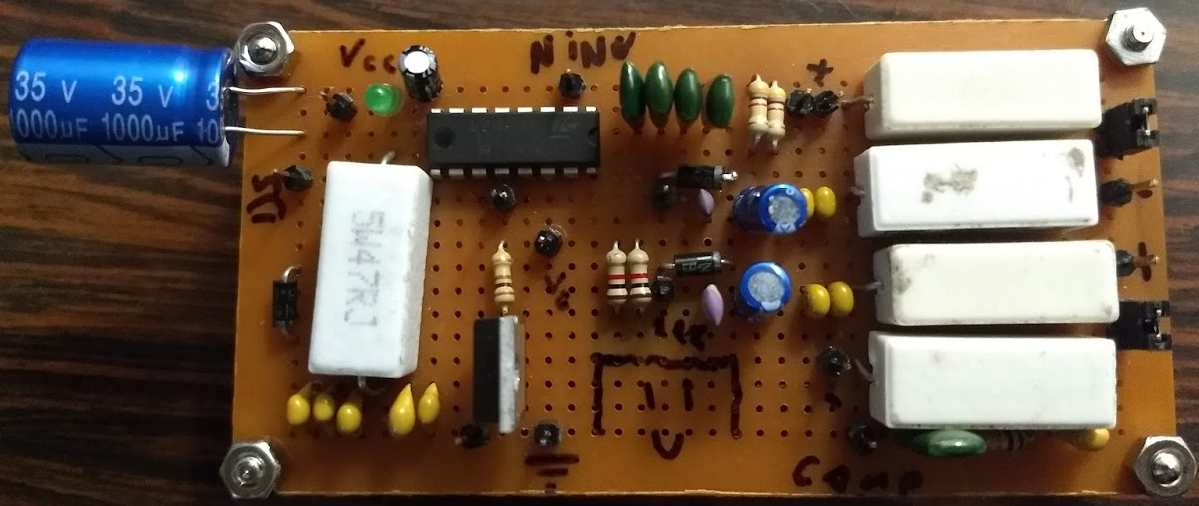
\includegraphics[width=0.7\linewidth]{ImagenesParteIV/placa_facha.png}
	\label{fig:vcom_4}
	\caption{Tensión de compensación.}
\end{figure}


\subsection{Mediciones}
Lo primero que vemos en la tensión de compensación que a diferencia de (\ref{fig:com3}) este cuenta con un valor menor debido a que se tiene una $V_{ref}$ distinta para obtener la salida deseada.
\begin{figure}[H]
	\centering
	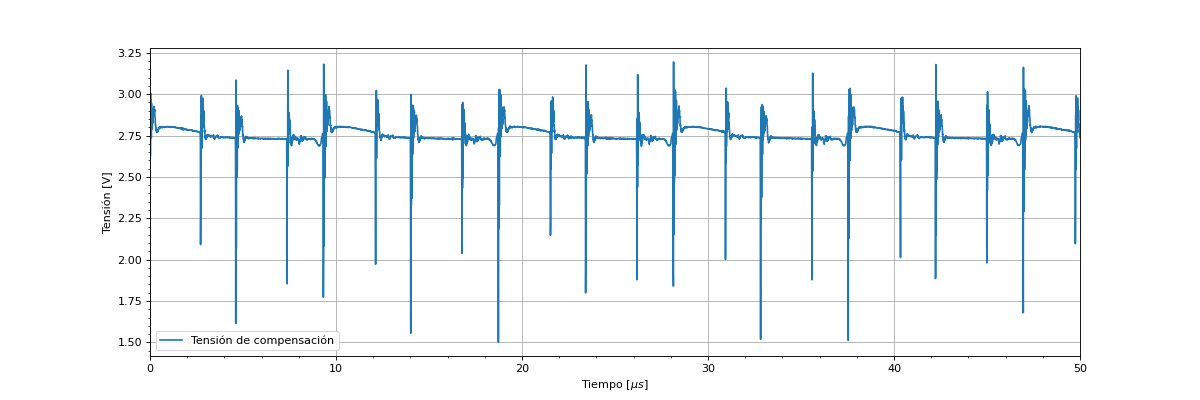
\includegraphics[width=0.9\linewidth]{ImagenesParteIV/Vcom.png}
	\label{fig:vcom_4}
	\caption{Tensión de compensación.}
\end{figure}
Se puede observar que la tensión en el capacitor de snubber efectivamente no se llega a descargar por completo debido a la selección de la resistencia de snubber limitado a la disponibilidad de componentes.
\begin{figure}[H]
	\centering
	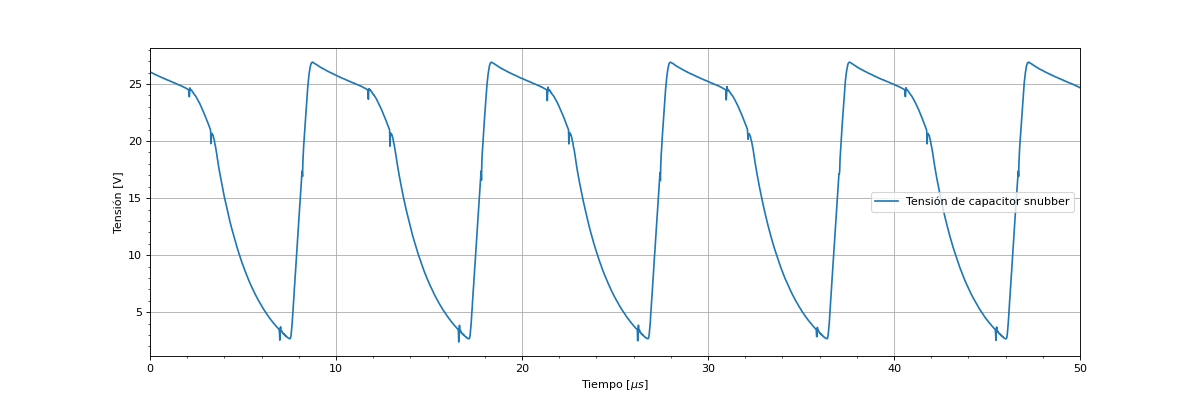
\includegraphics[width=0.9\linewidth]{ImagenesParteIV/Vcsnubber.png}
	\label{fig:vcsnubb_4}
	\caption{Tensión de capacitor de snubber.}
\end{figure}

\begin{figure}[H]
	\centering
	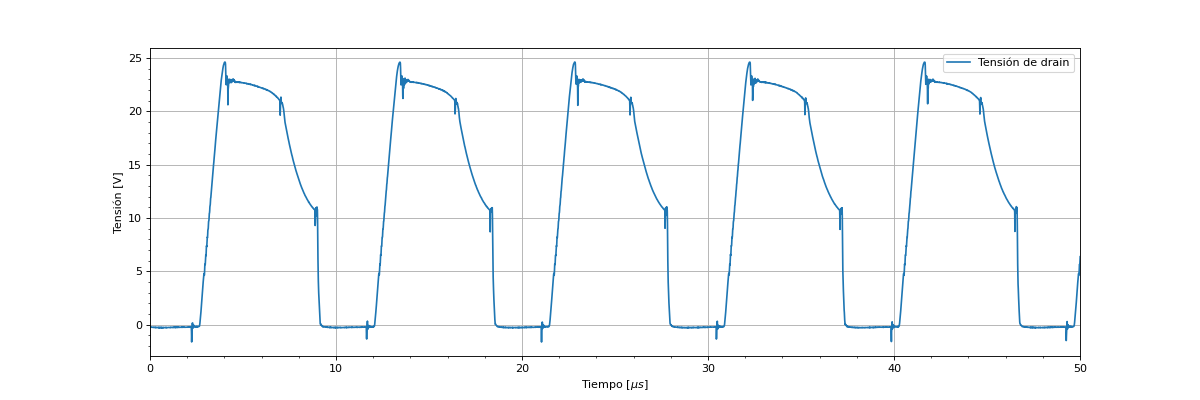
\includegraphics[width=0.9\linewidth]{ImagenesParteIV/Vds.png}
	\label{fig:vds_4}
	\caption{Tensión de drain.}
\end{figure}

\begin{figure}[H]
	\centering
	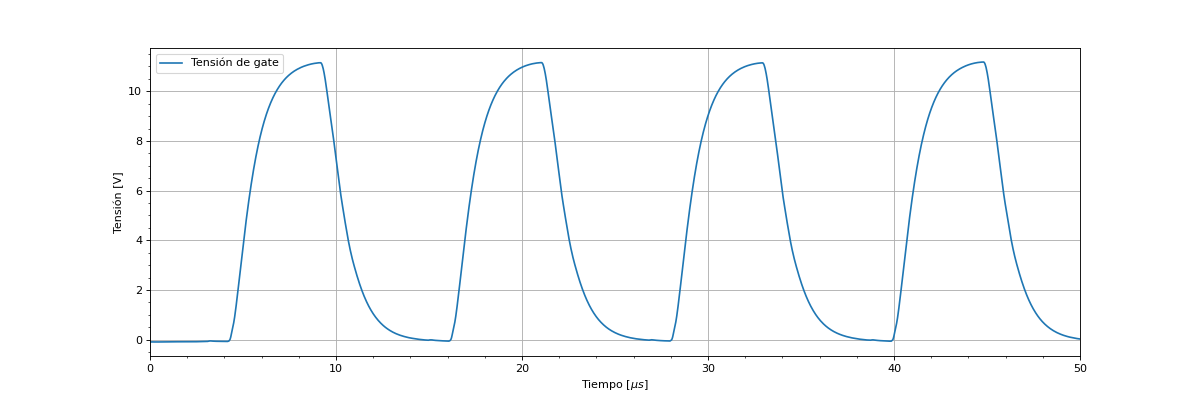
\includegraphics[width=0.9\linewidth]{ImagenesParteIV/Vgs.png}
	\label{fig:vgs_4}
	\caption{Tensión de gate.}
\end{figure}
Aquí se ve el terminal no inversor, la variación en la forma de onda se debe a la incapacidad del analog en mantener una tensión constante de 2V.
\begin{figure}[H]
	\centering	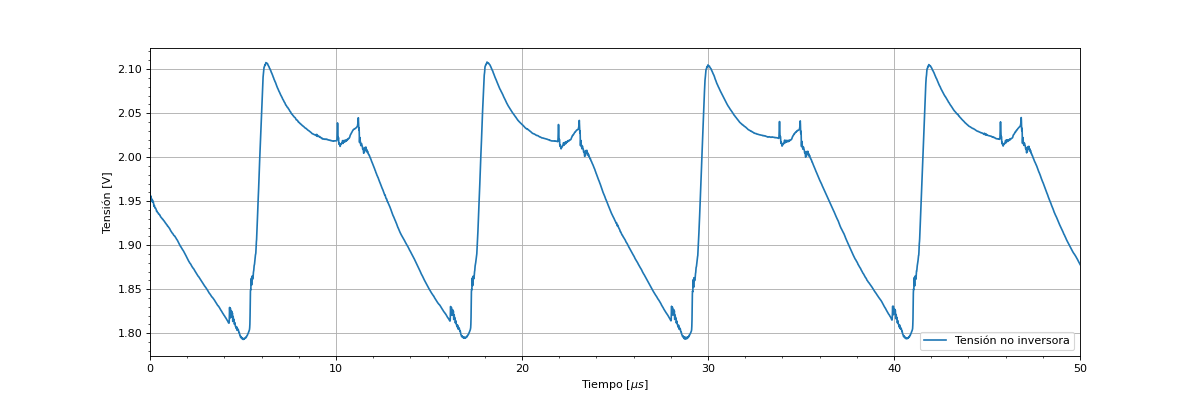
\includegraphics[width=0.9\linewidth]{ImagenesParteIV/Vni.png}
	\label{fig:vni_4}
	\caption{Tensión no inversora.}
\end{figure}

En la siguiente figura se ve  la tensión de salida, la cual se mantiene en el rango de tensiones permitido, teniendo un ripple de salida de aproximadamente el 5\%.  Aunque tiene unos picos de alta frecuencia que se dan en 4 ocaciones especificas que van a a ser explicadas luego.

\begin{figure}[H]
	\centering	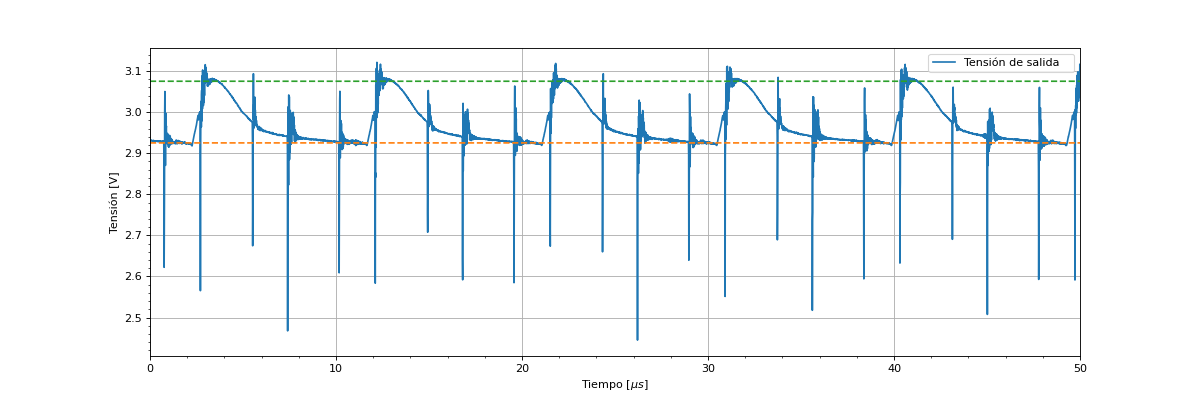
\includegraphics[width=0.9\linewidth]{ImagenesParteIV/Vout.png}
	\label{fig:vout_4}
	\caption{Tensión de salida.}
\end{figure}
\begin{figure}[H]
	\centering
	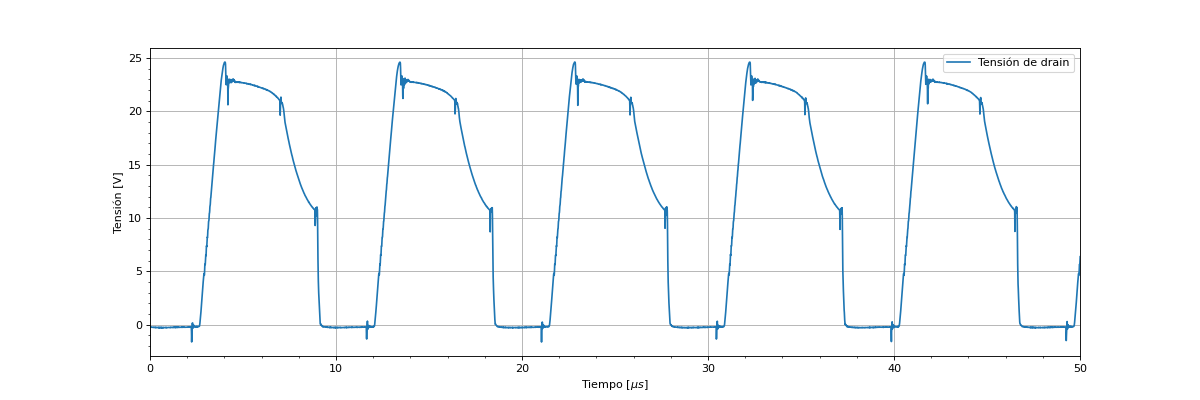
\includegraphics[width=0.9\linewidth]{ImagenesParteIV/Vds.png}
	\label{fig:vds_4}
	\caption{Tensión de drain.}
\end{figure}
\begin{figure}[H]
	\centering
	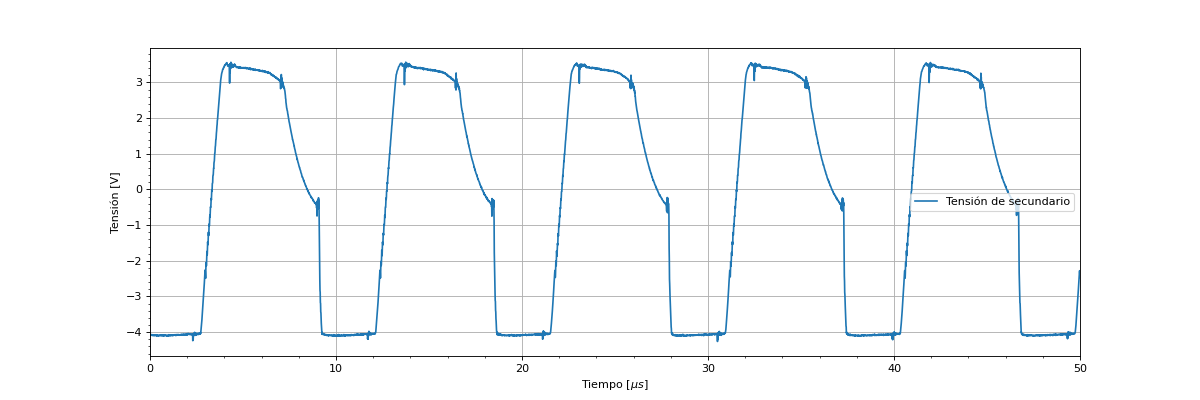
\includegraphics[width=0.9\linewidth]{ImagenesParteIV/Vsec.png}
	\label{fig:vsec_4}
	\caption{Tensión de secundario.}
\end{figure}
Se pueden observar cuatro oscilaciones distintivas en las mediciones de la mayoría de las tensiones del circuito, estas suceden al momento de apagar la llave, debido a los efectos de la $L_d$, inmediatamente después de apagar la llave provocado por el sobrepico del diodo de potencia. Al quedarse sin energía el núcleo del transformador por las mismas razones explicadas anteriormente. Y finalmente al encender la llave, aqui suceden 2 cosas el capacitor del snubber se descarga sobre el MOS al igual que se comienza a cargar la inductancia del primario.
%\end{document}